\documentclass[spanish,11pt,letterpaper]{article}

\usepackage[spanish]{babel}
\usepackage[utf8]{inputenc}
\usepackage{authblk}
\usepackage{amsmath}
\usepackage{amssymb}
\usepackage{amsthm}
\usepackage[margin=1in]{geometry}
\usepackage{graphicx}
\usepackage{hyperref}
% \usepackage{listings}
% \usepackage{xcolor}
\renewcommand{\vec}[1]{\mathbf{#1}}
\decimalpoint

\title{Clasificación de canciones por género en base a la música\\
usando aprendizaje colectivo}
\author{Hernández Chiapa David Felipe\\
López García Gilberto Isaac}
\affil{Facultad de Ciencias\\{\small Universidad Nacional Autónoma de México}}
\date{\small\today}

\begin{document}

\maketitle

\section{Introducción}

En el primer proyecto, \textit{Sistema de clasificación automática de documentos,
Clasificación de canciones por género con base en la letra}, atacamos el problema
de clasificación de canciones por género basándonos solo en la letra
asumiendo que el léxico usado determinaría el género. Esta
forma de enfrentar el problema no dió buenos resultados pues nuestros algoritmos
de clasificación tenía un porcentaje de acierto de entre 50 y 60 por ciento,
básicamente estaban adivinando al azar.

En el presente trabajo usaremos audio para la clasificación, usando un clasificador
colectivo compuesto de redes convolucionales sobre los espectrogramas de la música,
pues no solo la letra sino el sonido es necesario para determinar el género de
una pieza musical.

\section{Definición del problema}

\subsection{Espectrogramas}

Un espectrograma es una representación visual de una señal como el sonido, que
guarda información sobre el espectro de frecuencias y su variación en el tiempo.
Viendo el sonido como una función del tiempo, un espectrograma se puede obtener
mediante la Transformada de Fourier de esa señal, para obtener las frecuencias
que componen la señal y sus amplitudes. Esta información queda codificada como una
imagen donde cada pixel con coordenadas $(t,f)$, donde $t$ es una posición en el
tiempo (un intervalo pequeño pues la señal debe discretizarse para ser procesada
por la computadora) y $f$ una frecuencia, tiene un valor que corresponde a la
amplitud y se muestra como un color (ver Figura \ref{fig:specgram}).

\begin{figure}[h]
\centering
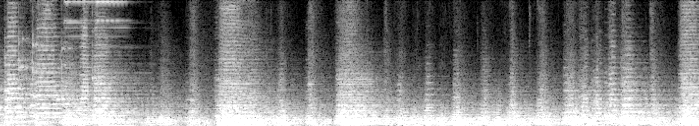
\includegraphics[width=0.9\textwidth]{specgram_classical.png}
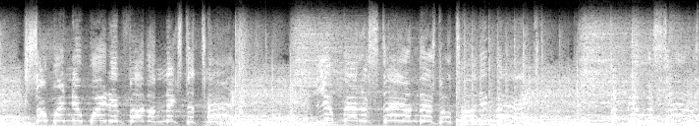
\includegraphics[width=0.9\textwidth]{specgram_metal.png}
\caption{Espectrograma de una canción `classical' (arriba) y `metal' (abajo).}
\label{fig:specgram}
\end{figure}

La amplitud puede estar en escala lineal o logarítmica (por ejemplo, decibeles).
Normalmente se escoge escala logarítmica, escala que usamos aquí.

Los espectrogramas son una representación muy usada para distintas tareas como
música, sonares, radares, procesamiento del habla, y en años recientes, para
identificar eventos en muestras de sonido como en \cite{audio_recognition}.

\section{Aprendizaje colectivo}

En el proyecto \textit{Is this Loss? Sistema de reconocimiento de objetos en
imágenes} ya se habló de las redes convolucionales por lo que aquí se omite su
discusión y procedemos a hablar de clasificadores colectivos.

El aprendizaje colectivo, en inglés \textit{ensemble learning}\footnote{Traducción
del término adoptada por los autores del presente escrito.}, es el proceso de usar
distintos modelos, ya sean clasificadores o expertos, generados y combinados
estratégicamente para lograr un mejor desempeño en tareas de predicción (clasificación
o regresión).

Un clasificador colectivo es un clasificador cuya predicción está en función de
las predicciones individuales de los modelos que lo componen. Se usan principalmente
para mejorar el desempeño individual de los modelos en conjunto, evitar seleccionar y trabajar
con un clasificador pobre y asignar una ``confianza'' a las decisiones hechas
por los modelos individuales\cite{scholarpedia}.

Aquí señalamos que el espacio de hipótesis es una combinación de los espacios
de los clasificadores individuales, pues un clasificador colectivo es una mezcla
finita de estos. En nuestro caso, usando cinco redes convolucionales, el espacio
de hipótesis es una mezcla del mismo espacio cinco veces.

\subsection{Bagging}

El clasificador colectivo que usaremos es \textit{Bagging}\footnote{Bootstrap
aggregation.}, un clasificador simple e intuitivo que ha demostrado tener un buen
desempeño (obviamente, esto si sus componentes tienen buen desempeño). Bagging
consiste en entrenar clasificadores independientemente sobre muestras aleatorias
con reemplazo del dataset y clasificar entradas por mayoría de votos en las
clasificaciones individuales de sus componentes. El algoritmo a continuación:\\
\textbf{Entrada:}
\begin{itemize}
  \item Conjunto de entrenamiento $S$ con conjunto de etiquetas
  $\{\ell_1,\ldots,\ell_m\}$ para $m$ clases distintas.
  \item Clasificadores que lo componen $C_1,\ldots,C_k$.
  \item Porcentaje $F$ de los datos que se usarán para entrenar a cada clasificador.
\end{itemize}
\textbf{Entrenamiento:} Para cada clasificador $C_i$:
\begin{enumerate}
  \item Tomar una muestra aleatoria con remplazo $S_i$ de $S$ con tamaño $F$ por
  ciento el tamaño de $S$.
  \item Entrenar el clasificador $C_i$ con el conjunto $S_i$.
\end{enumerate}
\textbf{Clasificación:} Dada una entrada $\vec{x}$:
\begin{enumerate}
  \item Evaluar cada clasificador $C_i$ con $\vec{x}$ para obtener una clase $y_i$.
  \item Para cada clase $\ell_1,\ldots,\ell_m$, contar el número de etiquetas
  resultantes de las predicciones de los clasificadores.
  \item La etiqueta $y$ para $\vec{x}$ es aquella clase que tuvo el mayor conteo
  en el paso anterior.
\end{enumerate}

\subsection{Intuición}

El propósito detrás de tomar subconjuntos $S_i$ para cada clasificador $C_i$ es
tener diversidad en lo aprendido por los clasificadores individualmente, y por lo
tanto, diversidad en sus respuestas. Tener diversidad en los componentes de un
clasificador colectivo nos ayuda a corregir errores hechos por algunos de estos;
los clasificadores cometen distintos errores en distintas entradas, pero en conjunto
deciden la ``mejor'' clasificación.

En este caso, usando bagging, la respuesta del clasificador colectivo no tiene
que ser la respuesta correcta, pero es la mejor respuesta en el sentido que
tuvo mayor cantidad de votos, esto es, el clasificador confía en que es la
respuesta correcta basado en las respuestas de sus componentes y el conocimiento
que tienen.

Si la gran mayoría de los clasificadores responden lo mismo decimos que el clasificador
colectivo tiene alta confianza en su respuesta, en otro caso, si las respuestas
no coinciden decimos que el clasificador tiene baja confianza en su respuesta.
Una respuesta con alta confianza no tiene por que ser correcta, y una con baja
confianza no tiene que ser incorrecta, pero si los componentes fueron propiamente
entrenados, en general una respuesta con alta confianza es correcta y con baja
confianza incorrecta\cite{scholarpedia}.

\subsection{Ventajas y desventajas}

Una ventaja de los clasificadores colectivos es, como ya se mencionó, la capacidad
de asignar una confianza a las respuestas que da; en el caso de \textit{bagging}
por mayoría de votos en los clasificadores individuales que han aprendido
distintas características de los datos. Como lo hacemos los humanos, un clasificador
colectivo responde con confianza que una muestra pertenece a cierta clase pues
sus componentes respondieron de la misma manera, como personas discutiendo
y concluyendo un resultado en base a conocimiento y experiencia personal que
en conjunto se complementa.

Como desventaja tenemos que entrenar múltiples clasificadores, posiblemente de
distinta naturaleza, puede ser una tarea difícil y computacionalmente costosa.
Por el lado de los datos esto puede representar una ventaja: si tenemos un dataset
de tamaño desmedido, cada clasificador se puede entrenar en un subconjunto de éste
de manera independiente, por lo que los clasificadores colectivos podrían ser
una buena opción cuando se traten problemas con grandes cantidades de datos. Más aún,
\textit{bagging} también aplica para pocos datos pues se basa principalmente en
muestras con reemplazo para generar los subconjuntos de entrenamiento
(\textit{bootstrap sampling}).

\section{Datos y preprocesamiento}

El dataset para el proyecto es \textsf{GTZAN Genre Collection}%
\footnote{\url{http://marsyasweb.appspot.com/download/data_sets/}}, que consiste de
una colección de 1000 clips de canciones con una duración de 30 segundos cada uno,
clasificados en 10 géneros musicales distintos: blues, classical, country, disco,
hiphop, jazz, metal, pop, reggae y rock, 100 clips por género.

Se obtuvo el espectrograma de estos clips, y estos espectrogramas (imágenes
\texttt{.png}) son los datos que se usaron para realizar una clasificación con
redes convolucionales.

Los espectrogramas obtenidos se pueden considerar como arreglos de 3 dimensiones: tiempo, frecuencia
y amplitud. A la amplitud aplicamos logaritmo base 10 para tener una escala en
decibeles. Los espectrogramas resultantes son imágenes de tamaño $127 \times 2900$,
127 frecuencias registradas en 2900 intervalos de tiempo.

\section{Implementación}

Para implementar las redes convolucionales nos basamos en el procedimiento descrito
en \cite{audio_recognition}. Las redes convolucionales trabajarán con las
imágenes de los espectrogramas de las canciones.

Creamos 5 redes convolucionales, con una capa de convolución de 100 filtros de
tamaño $127 \times 25$ en strides de 5 pixeles, y una capa de max pooling de tamaño
$1 \times 5$. Los filtros abarcan todo el alto de las imágenes pues solo
nos interesa analizar los datos en el flujo de tiempo, por lo que vemos todas
las frecuencias en ventanas de tiempo de longitud $25$.

Seguido tenemos otra capa convolucional con 64 filtros de tamaño 15 y strides de
5 pixeles con una capa de max pooling de tamaño 2 (los mapas de características
solo tienen una dimensión pues en la primera capa se toman todas las frecuencias).

Finalmente un perceptrón multicapa con arquitectura (128,128,10) donde la última
capa realiza la clasificación con la función \textit{softmax}. Buscamos minimizar
el error minimizando la entropía cruzada de la función de clasificación de la red
y la clasificación real de los datos.

Como regularización aplicamos dropout con un parámetro de 0.5 entre capas, esto
para evitar sobreajuste de las redes. Dropout consiste en ``silenciar'' neuronas
o campos receptivos durante el proceso feedforward, que a su vez afecta al
algoritmo backpropagation, dejando una red más dispersa durante el entrenamiento
evitando ajustar todos los parámetros de la red.
El parámetro 0.5 significa que se silenciará la mitad de las neuronas/campos
receptivos.

En \cite{audio_recognition} tienen una red con una única
capa convolucional pero los filtros tienen tamaño distinto $F \times s$ donde
$F$ es el número de frecuencias en los espectrogramas y $s$ varía de 3 hasta 25,
por cada tamaño son 100 filtros. Nosotros seguimos su idea de usar muchos
de filtros y ventanas de tiempo grandes para obtener características abstractas
de los expectrogramas.

La implementación se realizó en el lenguaje de programación \textsc{Python 3},
con el módulo \textsc{Keras} usando \textsc{TensorFlow} como backend.

\section{Experimentación}

Este clasificador esta dividido en 5 clasificadores más pequeños, cada uno es una red convolucional, pero con la
misma arquitectura, es decir, son homogéneos entre ellos. El entrenamiento se realizó con una biblioteca de
imágenes, las cuales corresponden a los espectrogramas de los clips de 30 segundos antes descritos, a estos se les
dió un tratamiento especial, todos los espectrogramas tienen las mismas dimensiones, esto es necesario por razones
de implementación.

El entrenamiento del clasificador colectivo se hace por partes, como en este caso se utilizó uno que esta
compuesto de cinco clasificadores que a su vez son redes convolucionales, cada una de estas redes se entrenan por
separado con diferentes subconjuntos del dataset completo, esto es lo que hace que tengan diferentes resultados a
pesar de ser la misma red en cuanto a arquitectura. Se comenzó con cien épocas para entrenar a cada red, pero
notamos un sobreajuste considerable, fuimos disminuyendo estas hasta que llegamos a que la mejor cantidad de
épocas fue de quince. Los resultados obtenidos en este entrenamiento se presentan a continuación.

\section{Resultados}

En el primer intento de entrenamiento que se probó (una capa convolucional, entrenamiento por cien épocas), se obtuvo un porcentaje de precisión del 6\%, las diferentes componentes de este también tenían una precisión muy baja. Después de hacer el ajuste del clasificador (agregar una segunda capa convolucional y quince épocas), se obtuvieron mejores resultados:
\begin{itemize}
\item Clasificador 1: 11\% de precisión
\item Clasificador 2: 12\% de precisión
\item Clasificador 3: 12\% de precisión
\item Clasificador 4: 12\% de precisión
\item Clasificador 5: 13\% de precisión
\end{itemize}

De esto se obtuvo una precisión del clasificador colectivo de 15.66\% del dataset de pruebas. A pesar de que el
desempeño de este clasificador no es lo esperado, este se ve bastante beneficiado al usar la decisión conjunta de
las redes, es decir la votación de si esta bien o mal clasificado. Se pensó en añadir mas redes al clasificador,
pero no se cree que esto mejore sustancialmente la precisión pero si nos puede ayudar a asegurar que cuando las
clasificaciones que hace, son correctas, en caso de acertar.

\section{Conclusiones}

Como conclusión de este proyecto, en conjunto con el primer proyecto realizado, podemos decir que un
espectrograma, ni solo la letra de canciones, son suficientes para poder encontrar un patrón en estas que ayuden a
distinguir los géneros a los que pertenecen. Esto por que existen patrones en los espectrogramas que se repiten
entre los distintos géneros que hace difícil encontrar patrones distintivos entre géneros. Por ejemplo, la música
electrónica y el rap/trap de hoy en día tiene una base muy fuerte con los bajos y estos se ven representados de
manera similar en los espectrogramas, esto se podría comprobar si se observara la matriz de confusión de los clasificadores individuales y del colectivo.

Hoy en día se tienen sistemas que ya clasifican música, pero solamente por canción y no por género. Un sistema en
especifico, Shazam, es capaz de reconocer canciones con el simple hecho de escucharla por pocos segundos. La
pregunta que se queda abierta es ¿se podrá reconocer el género con un acercamiento parecido al que tiene este
sistema, el cual se sabe que también usa redes neuronales?, creemos que sí, pero primero se debe detectar, de
alguna manera, si los géneros se parecen entre si y poder escoger características mejores y con base en esto poder
tomar un mejor curso de acción a la hora de clasificar.

\begin{thebibliography}{9}
\bibitem{scholarpedia}
Ensemble Learning. (2009). Obtenido de
\url{http://www.scholarpedia.org/article/Ensemble_learning}

\bibitem{audio_recognition}
Phan, H., Hertel, L., Maass, M., \& Mertins, A. (2016).
Robust Audio Event Recognition with 1-Max Pooling Convolutional Neural Networks.
arXiv:1604.06338v2

\end{thebibliography}


\end{document}
